\section{プログラミングとは}
プログラミングとは,人間の意図した処理を行うようにコンピュータに指示を与える行為である.現在,身近にある様々なものはプログラムに従い動作している.コンピュータやスマートフォンはもちろん,炊飯器や洗濯機,自動車や信号機などを動かしているのもプログラムである.コンピュータは人間と違い,指示された通りのことしかできない.プログラミングはコンピュータに対して,「こうだったら,こうする」といった振る舞いのマニュアルを作成する行為であると言える.


\section{プログラミングを学習するメリット}
プログラミングを学ぶことで得られるメリットとして,作業の「効率化」が挙げられる.コンピュータは指示されたことしか実行できない代わりに,人間より高速かつ正確に処理を行うことができる.市販のコンピュータでさえ,1秒間に10億回の計算を行うことができる.プログラムを書くことができれば,人間が時間をかけてやっている面倒な作業を,コンピュータに任せることができるというメリットがある.


\section{Python}


\subsection{Pythonとは}
Pythonとは,簡潔で読みやすい文法が特徴的なプログラミング言語の一つである.プログラムの可読性が高くなるように設計されているので,CやJavaなどの言語に比べてより少ないコード行数でプログラムを表現することができる.GoogleやNASAの内部で利用されているという実績があり,本格的なプログラミングにも対応できる言語である.


\subsection{インタープリタ}
プログラムをコンピュータが理解できるマシン語(バイナリ)に変換するには,インタープリタとコンパイラという2種類の方式がある.Pythonはプログラムのソースコードを1行読み込むたびにマシン語に変換し実行するインタープリタ型の言語である.C言語やJavaはソースコード全体をマシン語に翻訳してから実行するコンパイラ型の言語である.インタープリタ型の言語はコンパイラ型の言語に比べて実行が遅いという欠点がある.その反面,1行ずつ処理を確認することができるので,プログラミング学習に向いていると言える.


\subsection{対話モード}
Pythonには,対話的にプログラムを入力,実行できる対話モードがある.対話モードを利用することで,1行ずつソースコードを打ち込み,その都度実行結果を確認することができる.


対話モードを利用するためには,Windowsの場合はコマンドプロンプトを,Macの場合はターミナルを起動し,``python''と入力することで起動することができる.


\begin{lstlisting}[caption=対話モード,label=interactive_mode]
$ python #コマンドプロンプトorターミナルでpythonと入力
Python 2.7.5 (default, Nov 20 2015, 02:00:19) #Pythonのバージョン情報など
[GCC 4.8.5 20150623 (Red Hat 4.8.5-4)] on linux2
Type "help", "copyright", "credits" or "license" for more information.
>>> #ユーザの入力を待ち受けるプロンプト
\end{lstlisting}

対話モードを起動した際のシェルの状態をソースコード\ref{interactive_mode}に示す.Pythonを対話モードで起動すると,バージョン情報などが表示された後に「\textgreater\textgreater\textgreater」という文字列が表示される.これはプロンプトと呼ばれるもので,Pythonがユーザの入力を待ち受けている状態であることを表す.


対話モードを終了したいときには,プロンプトが表示されている状態で``exit()''と入力するか,``Ctrl-D''キーを打ち込むことで終了できる.


\section{Hello World}
大抵のプログラミング言語で最初の例題とされているHello Worldについて解説する.


\begin{lstlisting}[caption=C言語のHello World,label=hello_C]
#include <stdio.h>
 
int main(void)
{
    printf("Hello world!");
    return 0;
}
\end{lstlisting}


\begin{lstlisting}[caption=PythonのHello World,label=hello_Python]
print "Hello World"
\end{lstlisting}


C言語のHello World(ソースコード\ref{hello_C})とPythonのHello World(ソースコード\ref{hello_Python})を比較すると,コード量の差がわかる.二つのプログラムは同じ処理をしている.C言語はPythonに比べて処理速度が早いというメリットがあるが,文法的な制約が多く,簡単な処理でもコード量が多くなってしまう.Pythonは文法的な制約が少ないので,簡潔に処理を書くことができる.


Pythonプログラムの ``print''は,半角スペースの後に続く文字列を出力するという命令である.Pythonでは文字列はダブルクオートかシングルクオートで囲むことで表現する.


\section{変数と代入}
変数とはプログラムの中で扱われるデータを記憶し,必要なときに利用するために,データに固有の名前を与えたものである.例えば,ある計算の結果をまた別の計算に再利用したい時などに用いる事ができる.変数に実際のデータを関連付けることを代入という.


\begin{lstlisting}[caption=変数と代入,label=var&assign]
>>> x = 3 #変数xに3を代入
>>> x + 5 #変数xには3が代入されているので,3+5となる
8 #3+5の計算結果が出力される
\end{lstlisting}


\begin{figure}[htbp]
\begin{center}
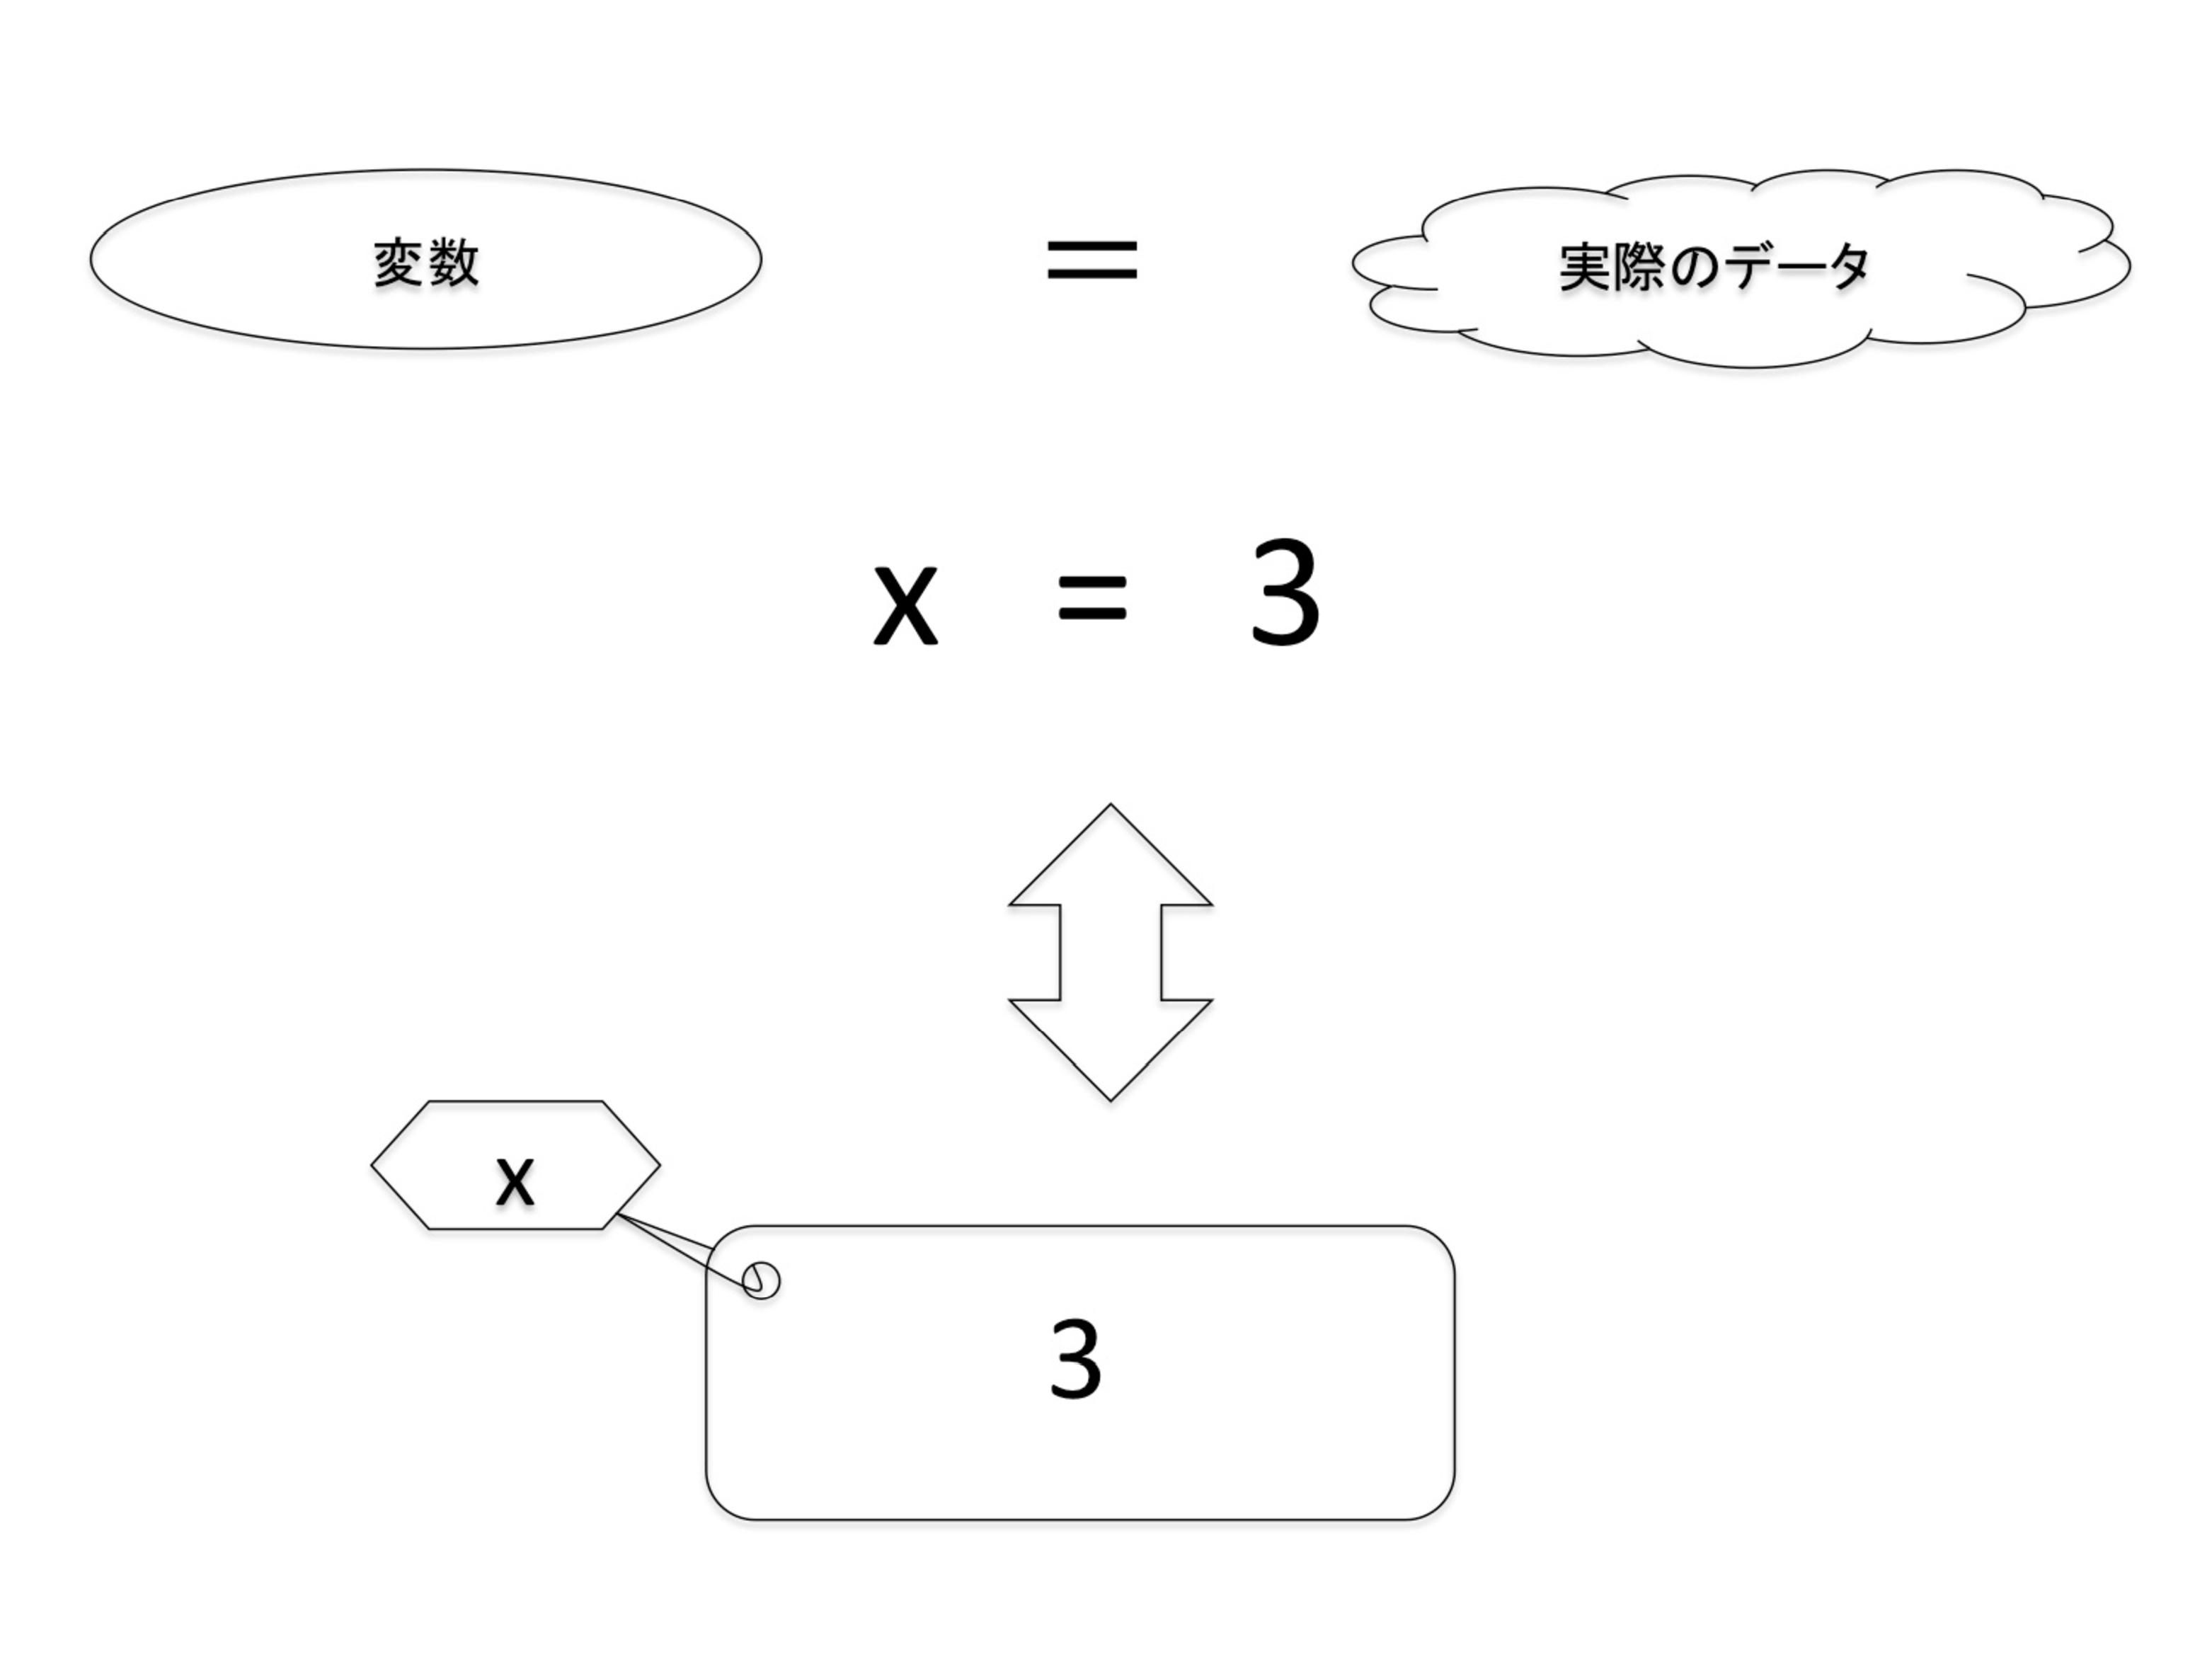
\includegraphics[width=9cm,bb=0 0 1500 1125]{var.pdf}
\caption{変数と代入のイメージ}
\label{fig:fig1}
\end{center}
\end{figure}


変数に使うことができる文字の種類は,アルファベット,数字,アンダースコアだけである.また,変数名はアルファベットの大文字と小文字が区別される.そのためxyzとXYZは違う変数となる.さらに数字を変数名の先頭に使うことはできない.


この他,予約語と呼ばれる特別な単語は,変数として利用できない.予約語の例を表\ref{tab:tab1}に示す.


\begin{table}[h]
  \begin{center}
  \caption{予約語}
  \begin{tabular}{|c|c|c|c|c|} \hline
  and & as & assert & break & class \\ \hline
  continue & def & del & elif & else \\ \hline
  except & exec & finally & for & from \\ \hline
  global & if & import & in & is \\ \hline
  lambda & not & or & pass & print \\ \hline
  raise & return & try & while & with \\ \hline
  yield & & & & \\ \hline
  \end{tabular}
  \label{tab:tab1}
  \end{center}
\end{table}


\section{標準入力}
世の中に存在するプログラムはすべて,なんらかのデータの入力を受け,そのデータを処理し,結果を出力する.例えば,電卓はユーザからの数値・演算子の入力,計算処理,結果の出力という流れで出来ている.


\begin{figure}[htbp]
\begin{center}
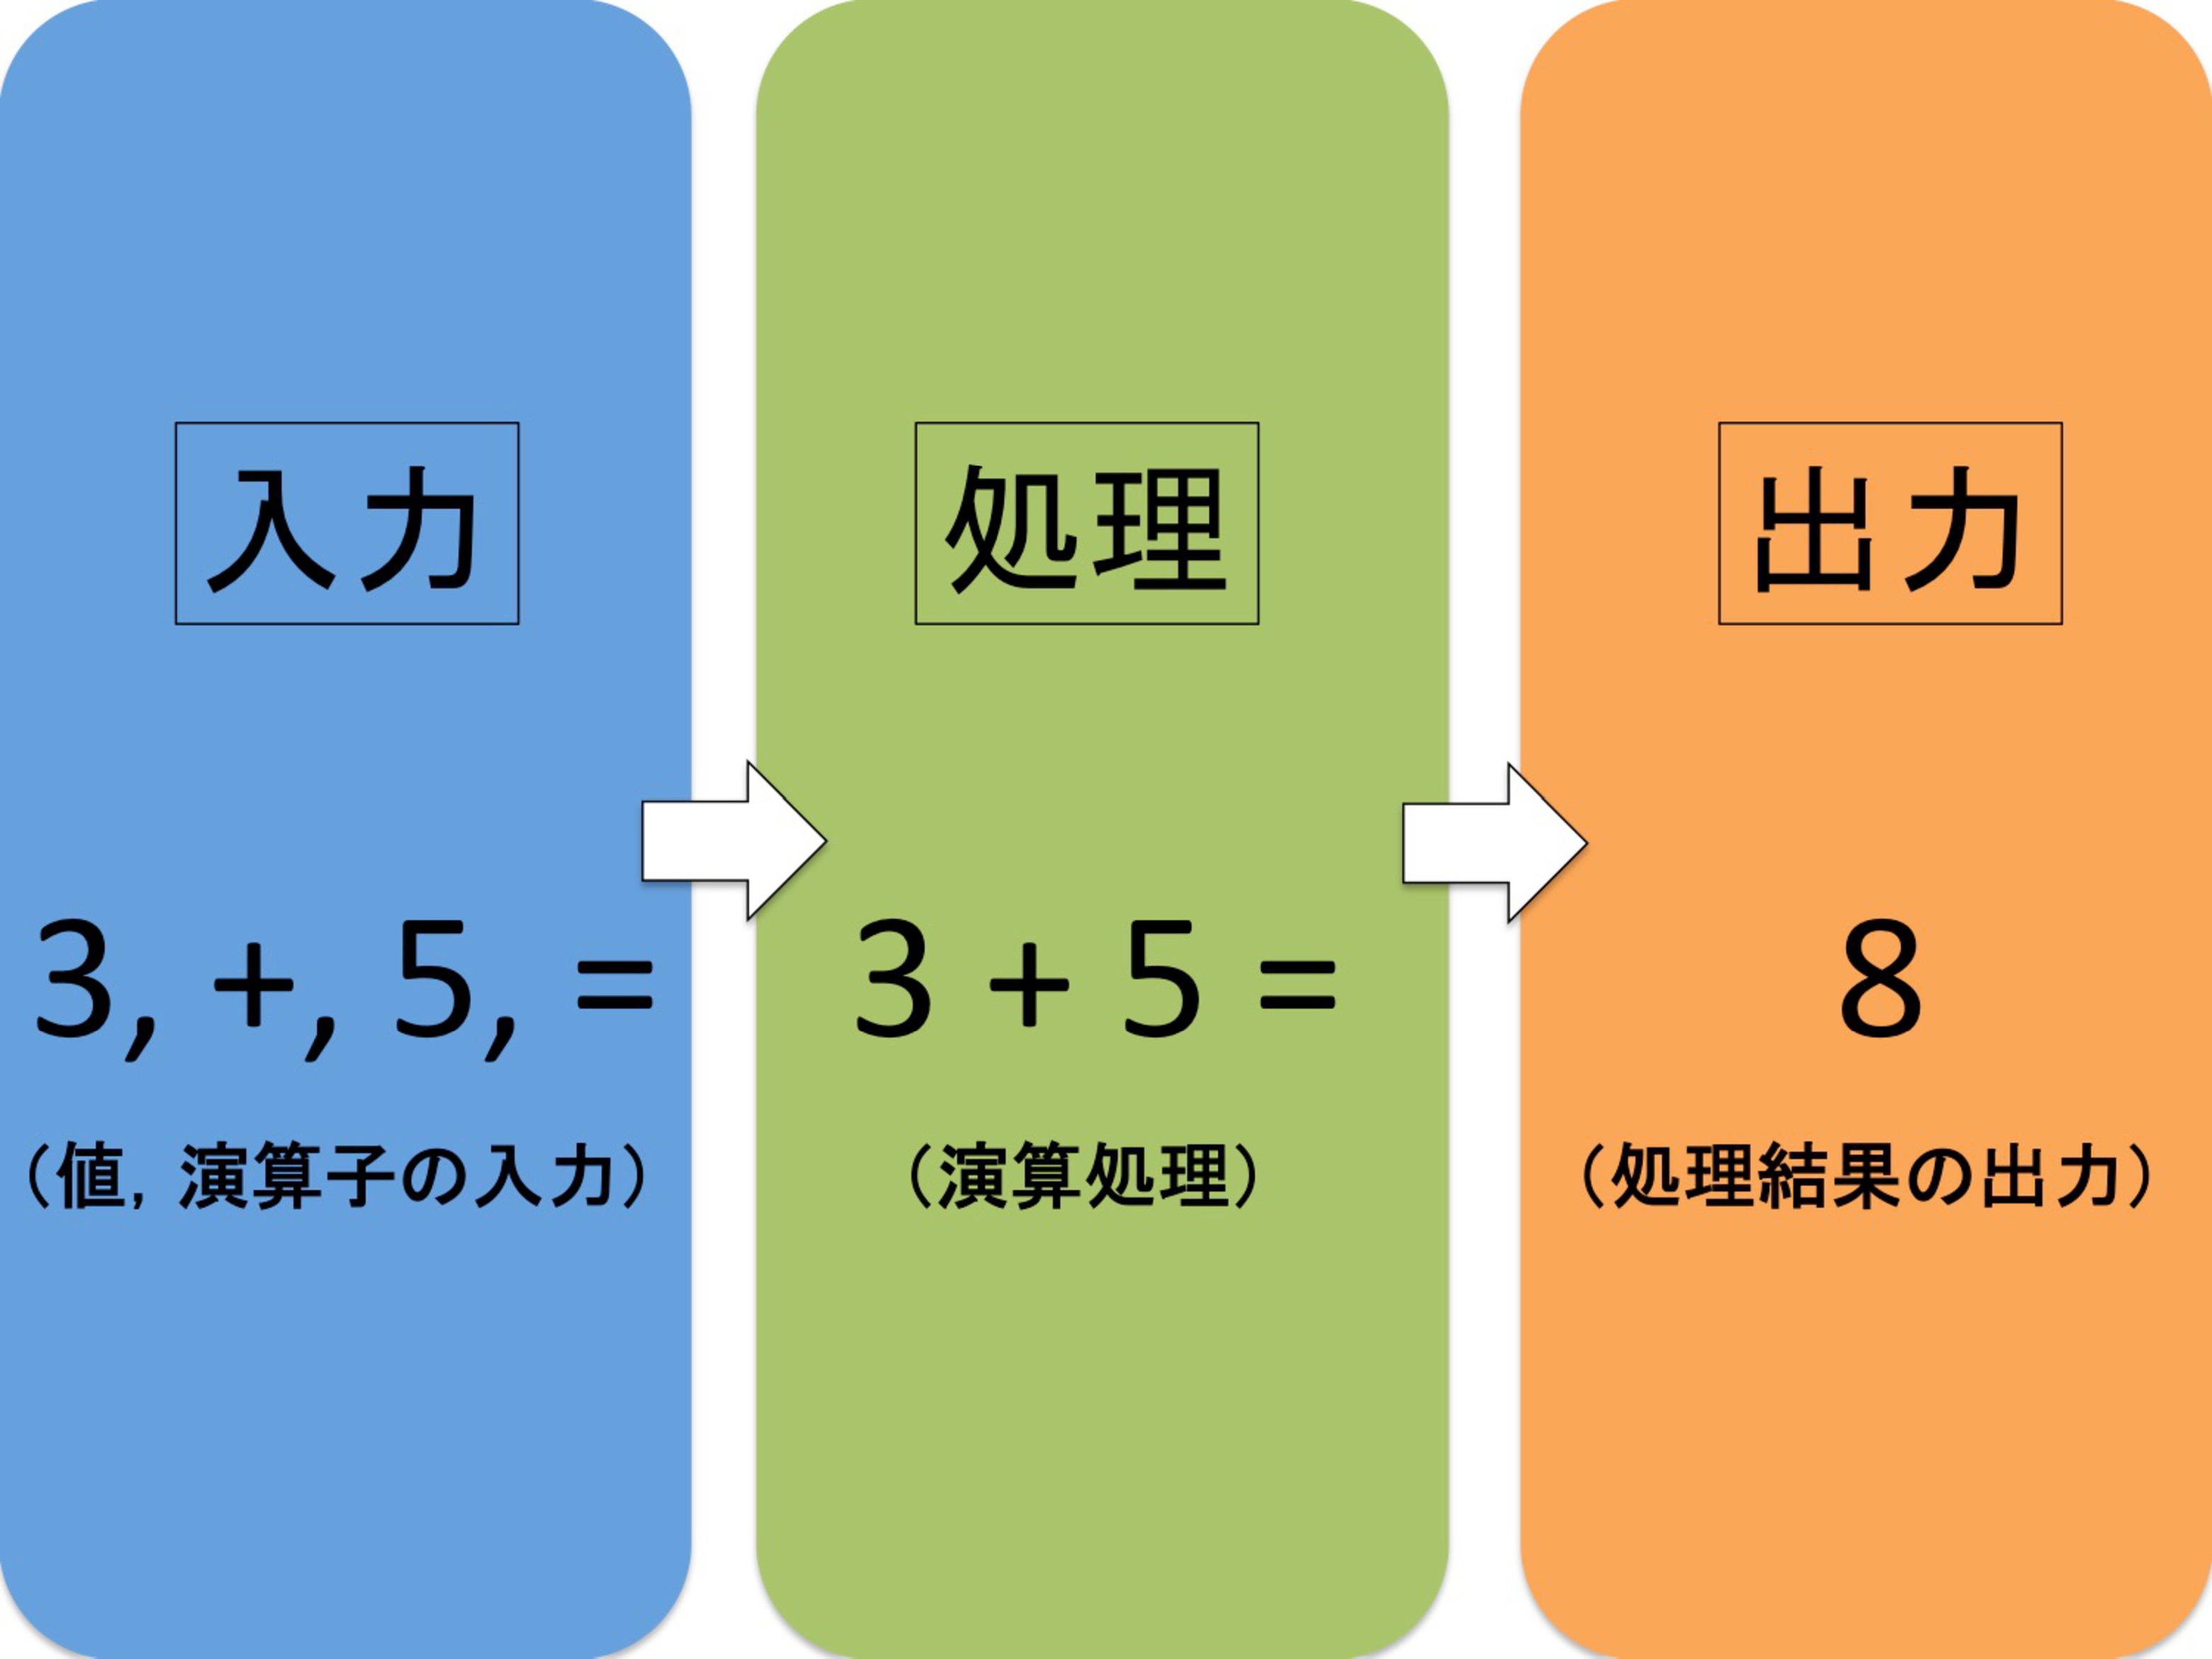
\includegraphics[width=9cm,bb=0 0 1500 1125]{calc.pdf}
\caption{電卓の入出力のイメージ}
\label{fig:fig2}
\end{center}
\end{figure}


入力はユーザがキーボードやマウスから行う場合もあれば,他のプログラムや,ファイルから読み込むこともある.プログラムに対して,キーボードから値を入力する仕組みを標準入力という.Pythonにおける標準入力の方法をソースコード\ref{std_input}に示す.


\begin{lstlisting}[caption=標準入力,label=std_input]
>>> input() #入力された値を式として扱う標準入力
3+5 #ユーザが入力した値
8 #入力された式を演算した結果

>>> raw_input() #入力された値を文字列として扱う標準入力
3+5 #ユーザが入力した値
'3+5' #入力された値を文字列として出力
\end{lstlisting}


1行目の``raw\_input''で,コマンドラインからの入力を取得している.Pythonの標準入力は2種類存在し,``raw\_input''は文字列の入力を受け付け,と``input''は式の入力を受け付ける.
